\section*{Wyniki}

Niniejszy rozdział stanowi prezentację wyników. Wykonaliśmy łącznie 3 eksperymenty, każdy dla 3 rozmiarów danych. Wyniki w każdym przypadku zostały uśrednione dla 3 przebiegów. Na każdym wykresie przedstawiono wagę drzewa dla przeciętnego osobnika w populacji. Os X stanowi ilość ewaluacji funkcji celu.

Poniższe trzy wykresy stanowią przypadek porównawczy dla zwykłego algorytmu genetycznego z selekcją turniejową.

Mały rozmiar danych:

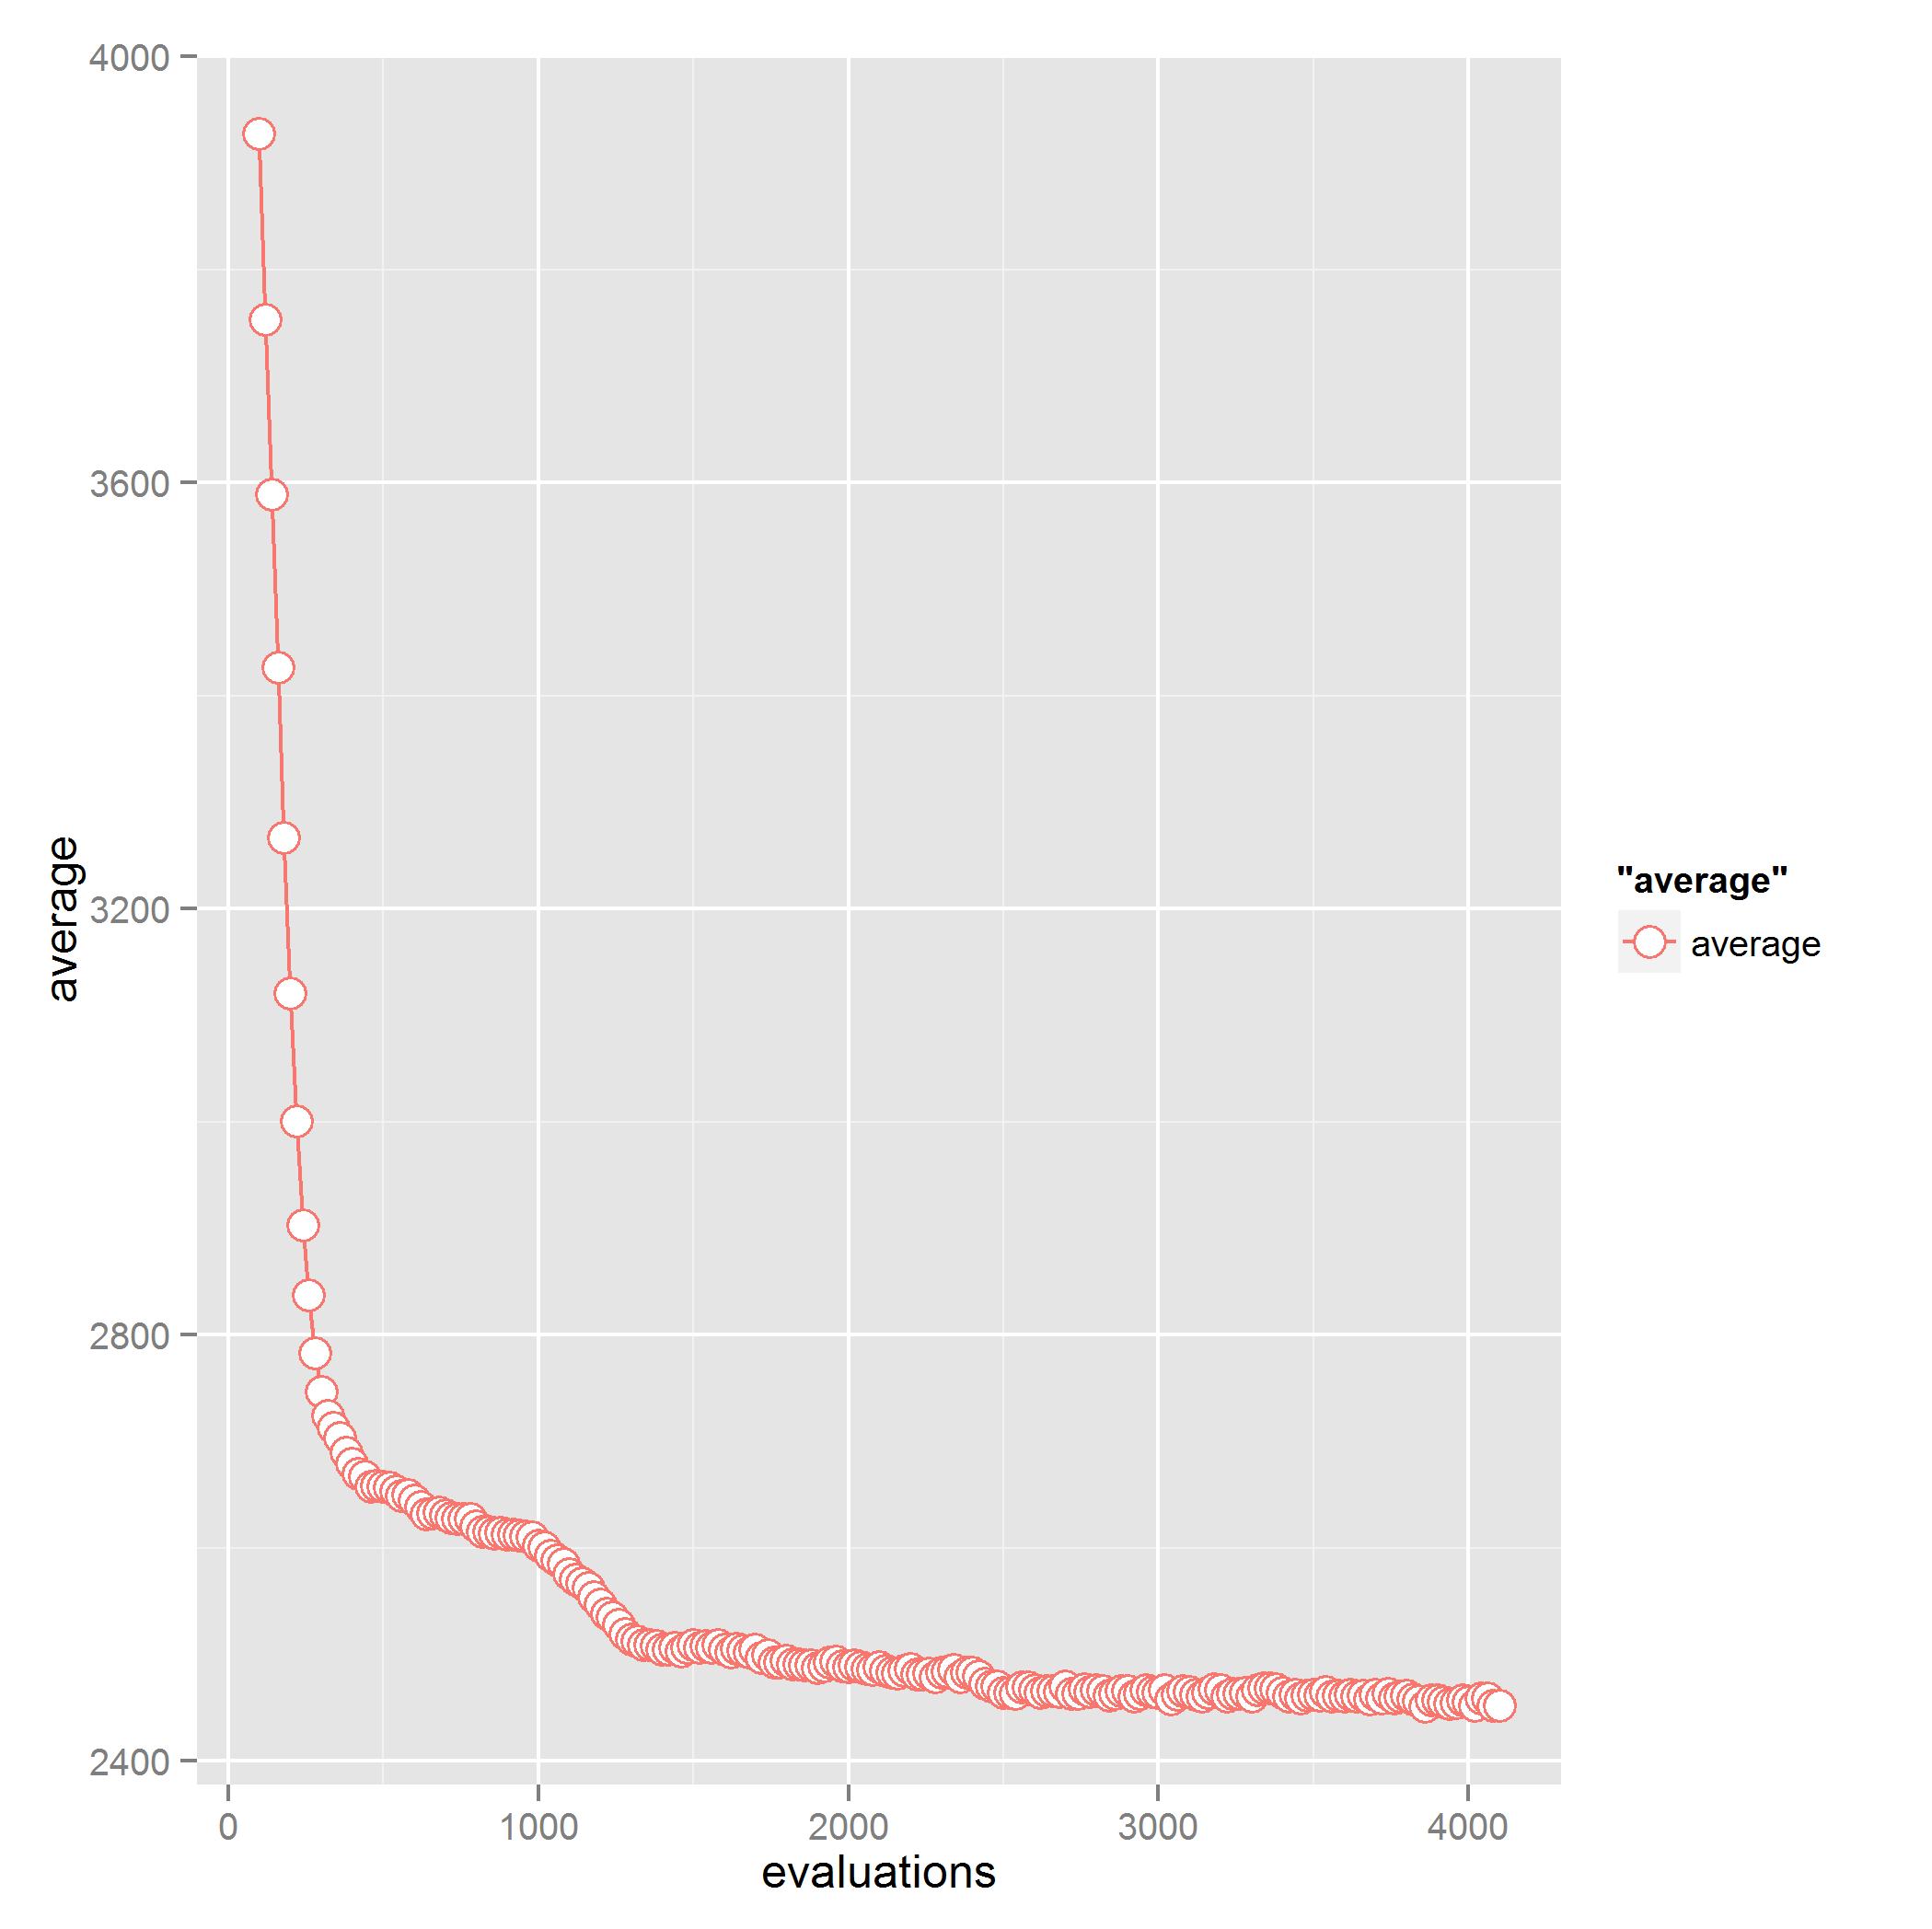
\includegraphics[]{simple_graph0.png}

Średni rozmiar danych:

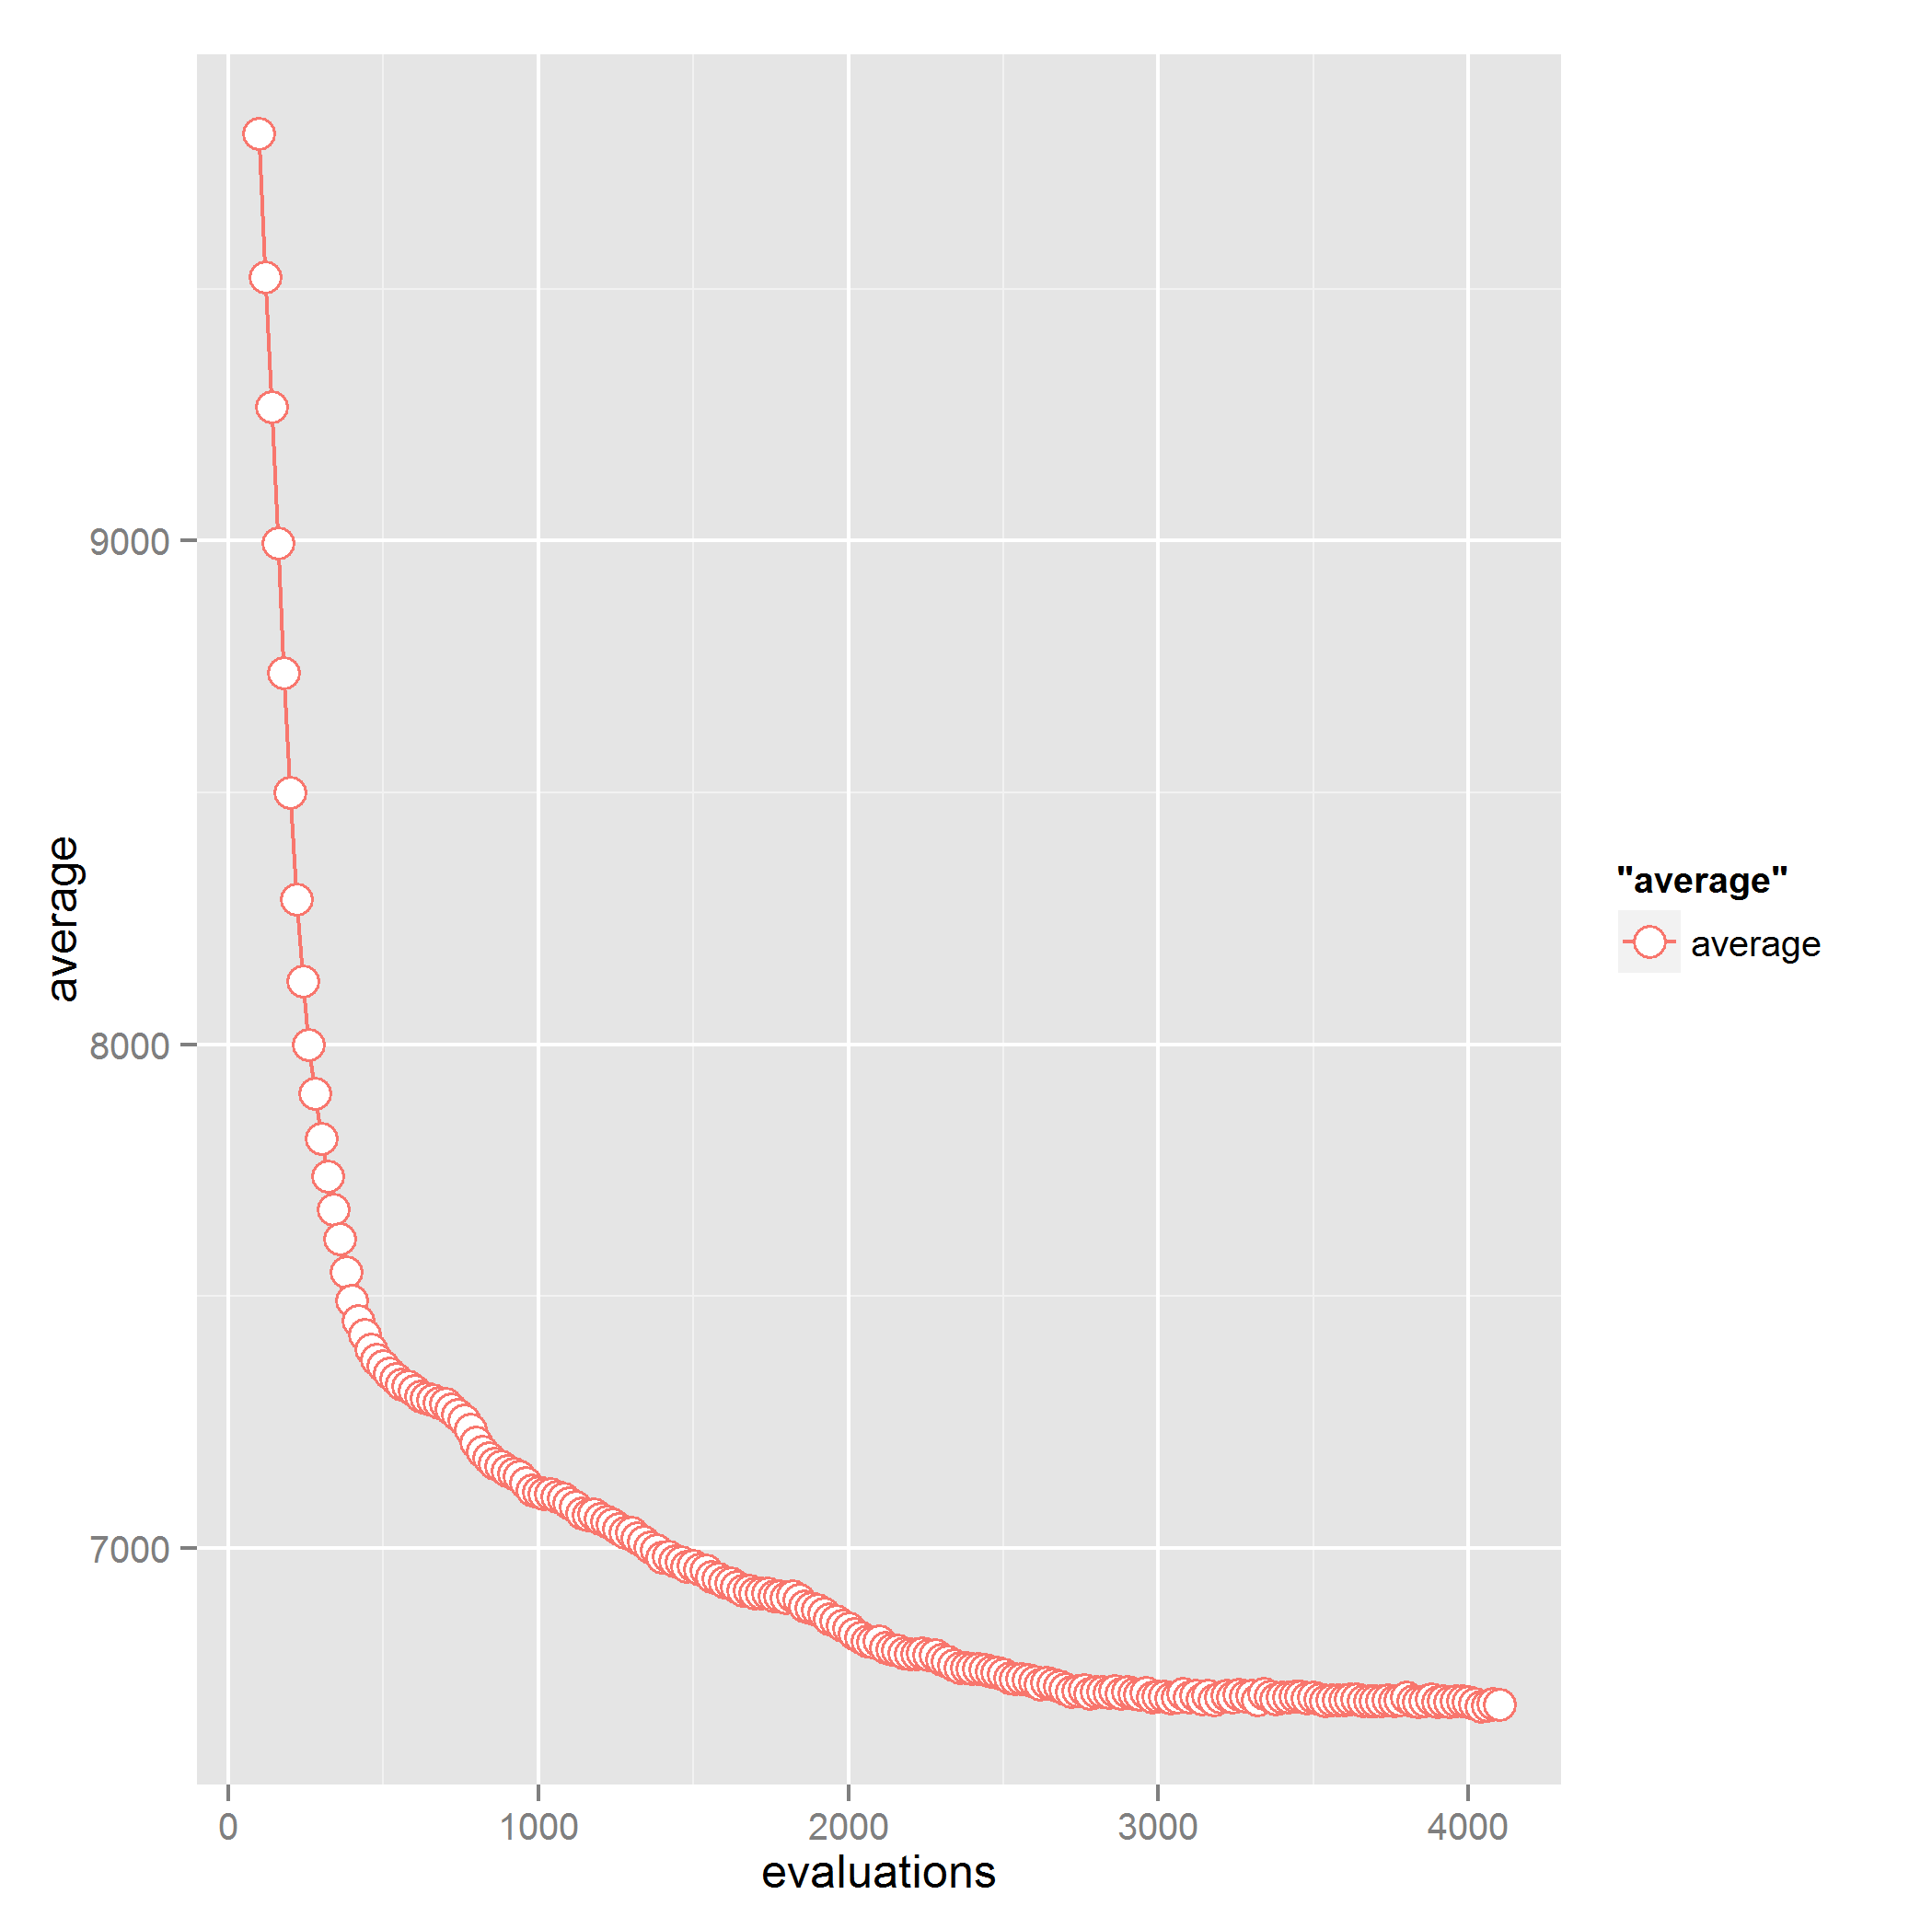
\includegraphics[]{simple_graph1.png}

Duży rozmiar danych:

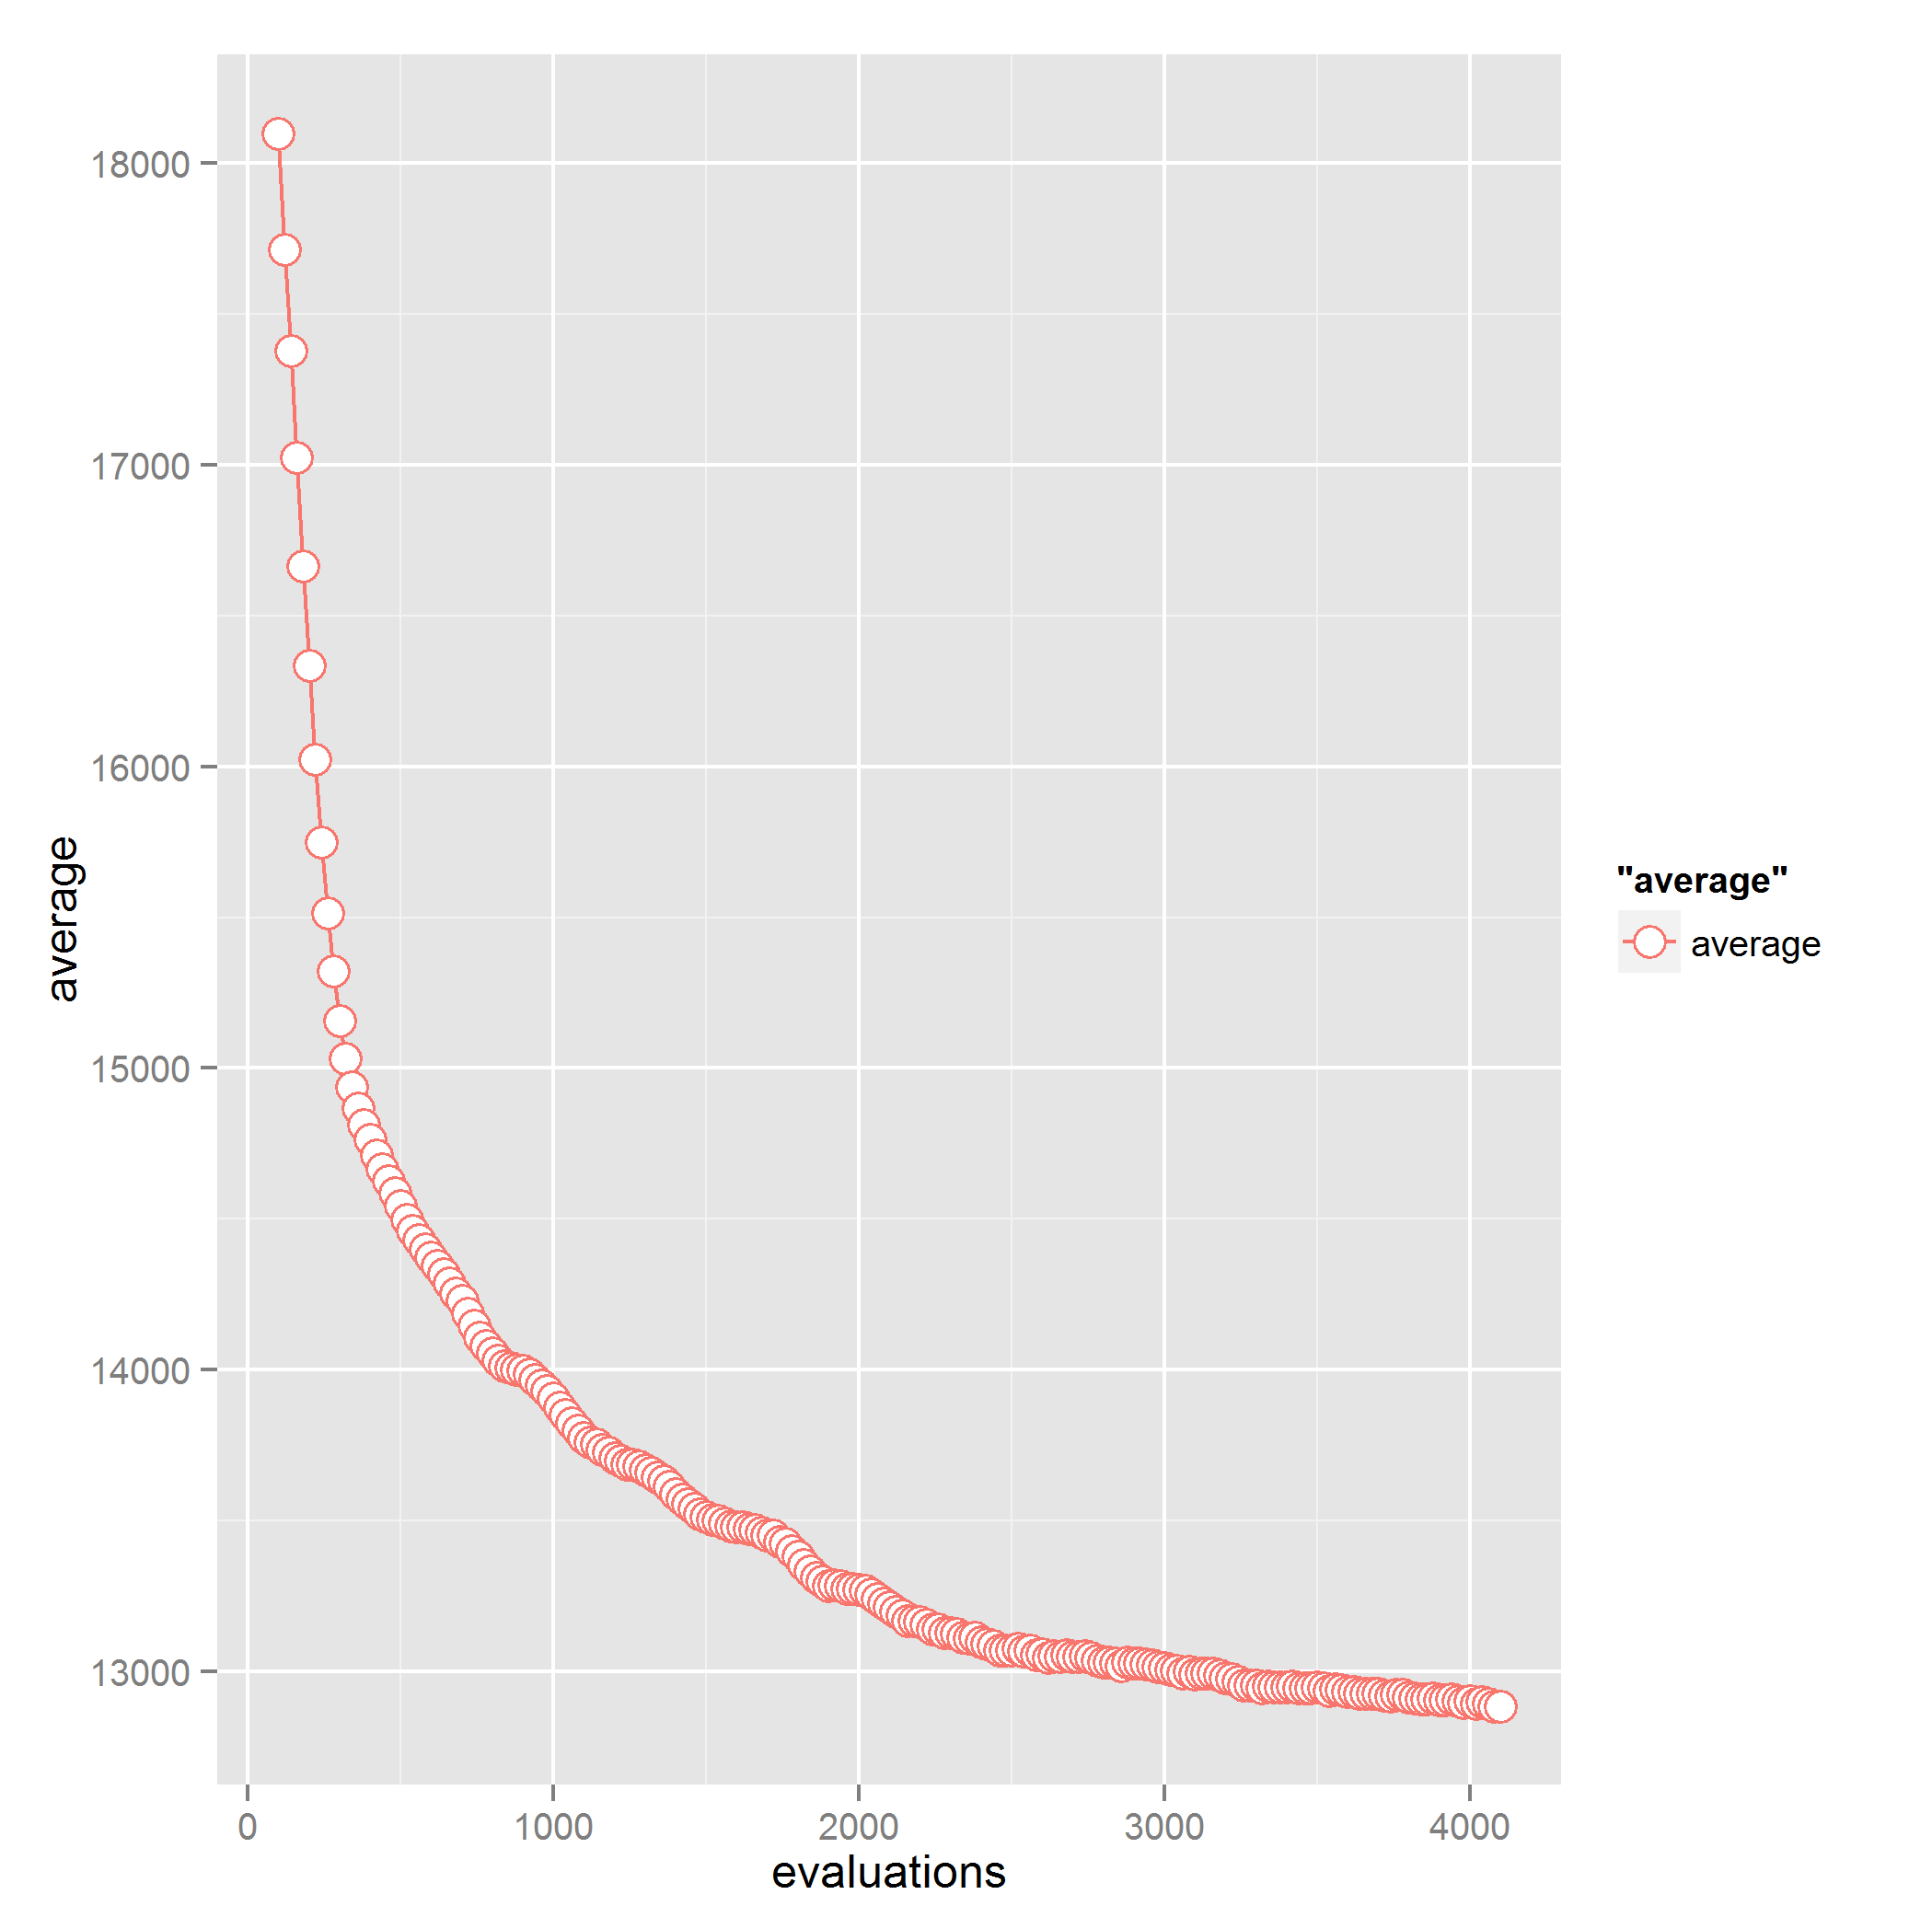
\includegraphics[]{simple_graph2.png}

Kolejne wyniki pochodzą z hybrydy algorytmu symulowanego wyżarzania, gdzie wychładzamy prawdopodobieństwo mutacji, które na początku miało dużą wartość np 1, a następnie jest wychładzane wykładniczo do bardzo małej wartości.

Mały rozmiar danych:

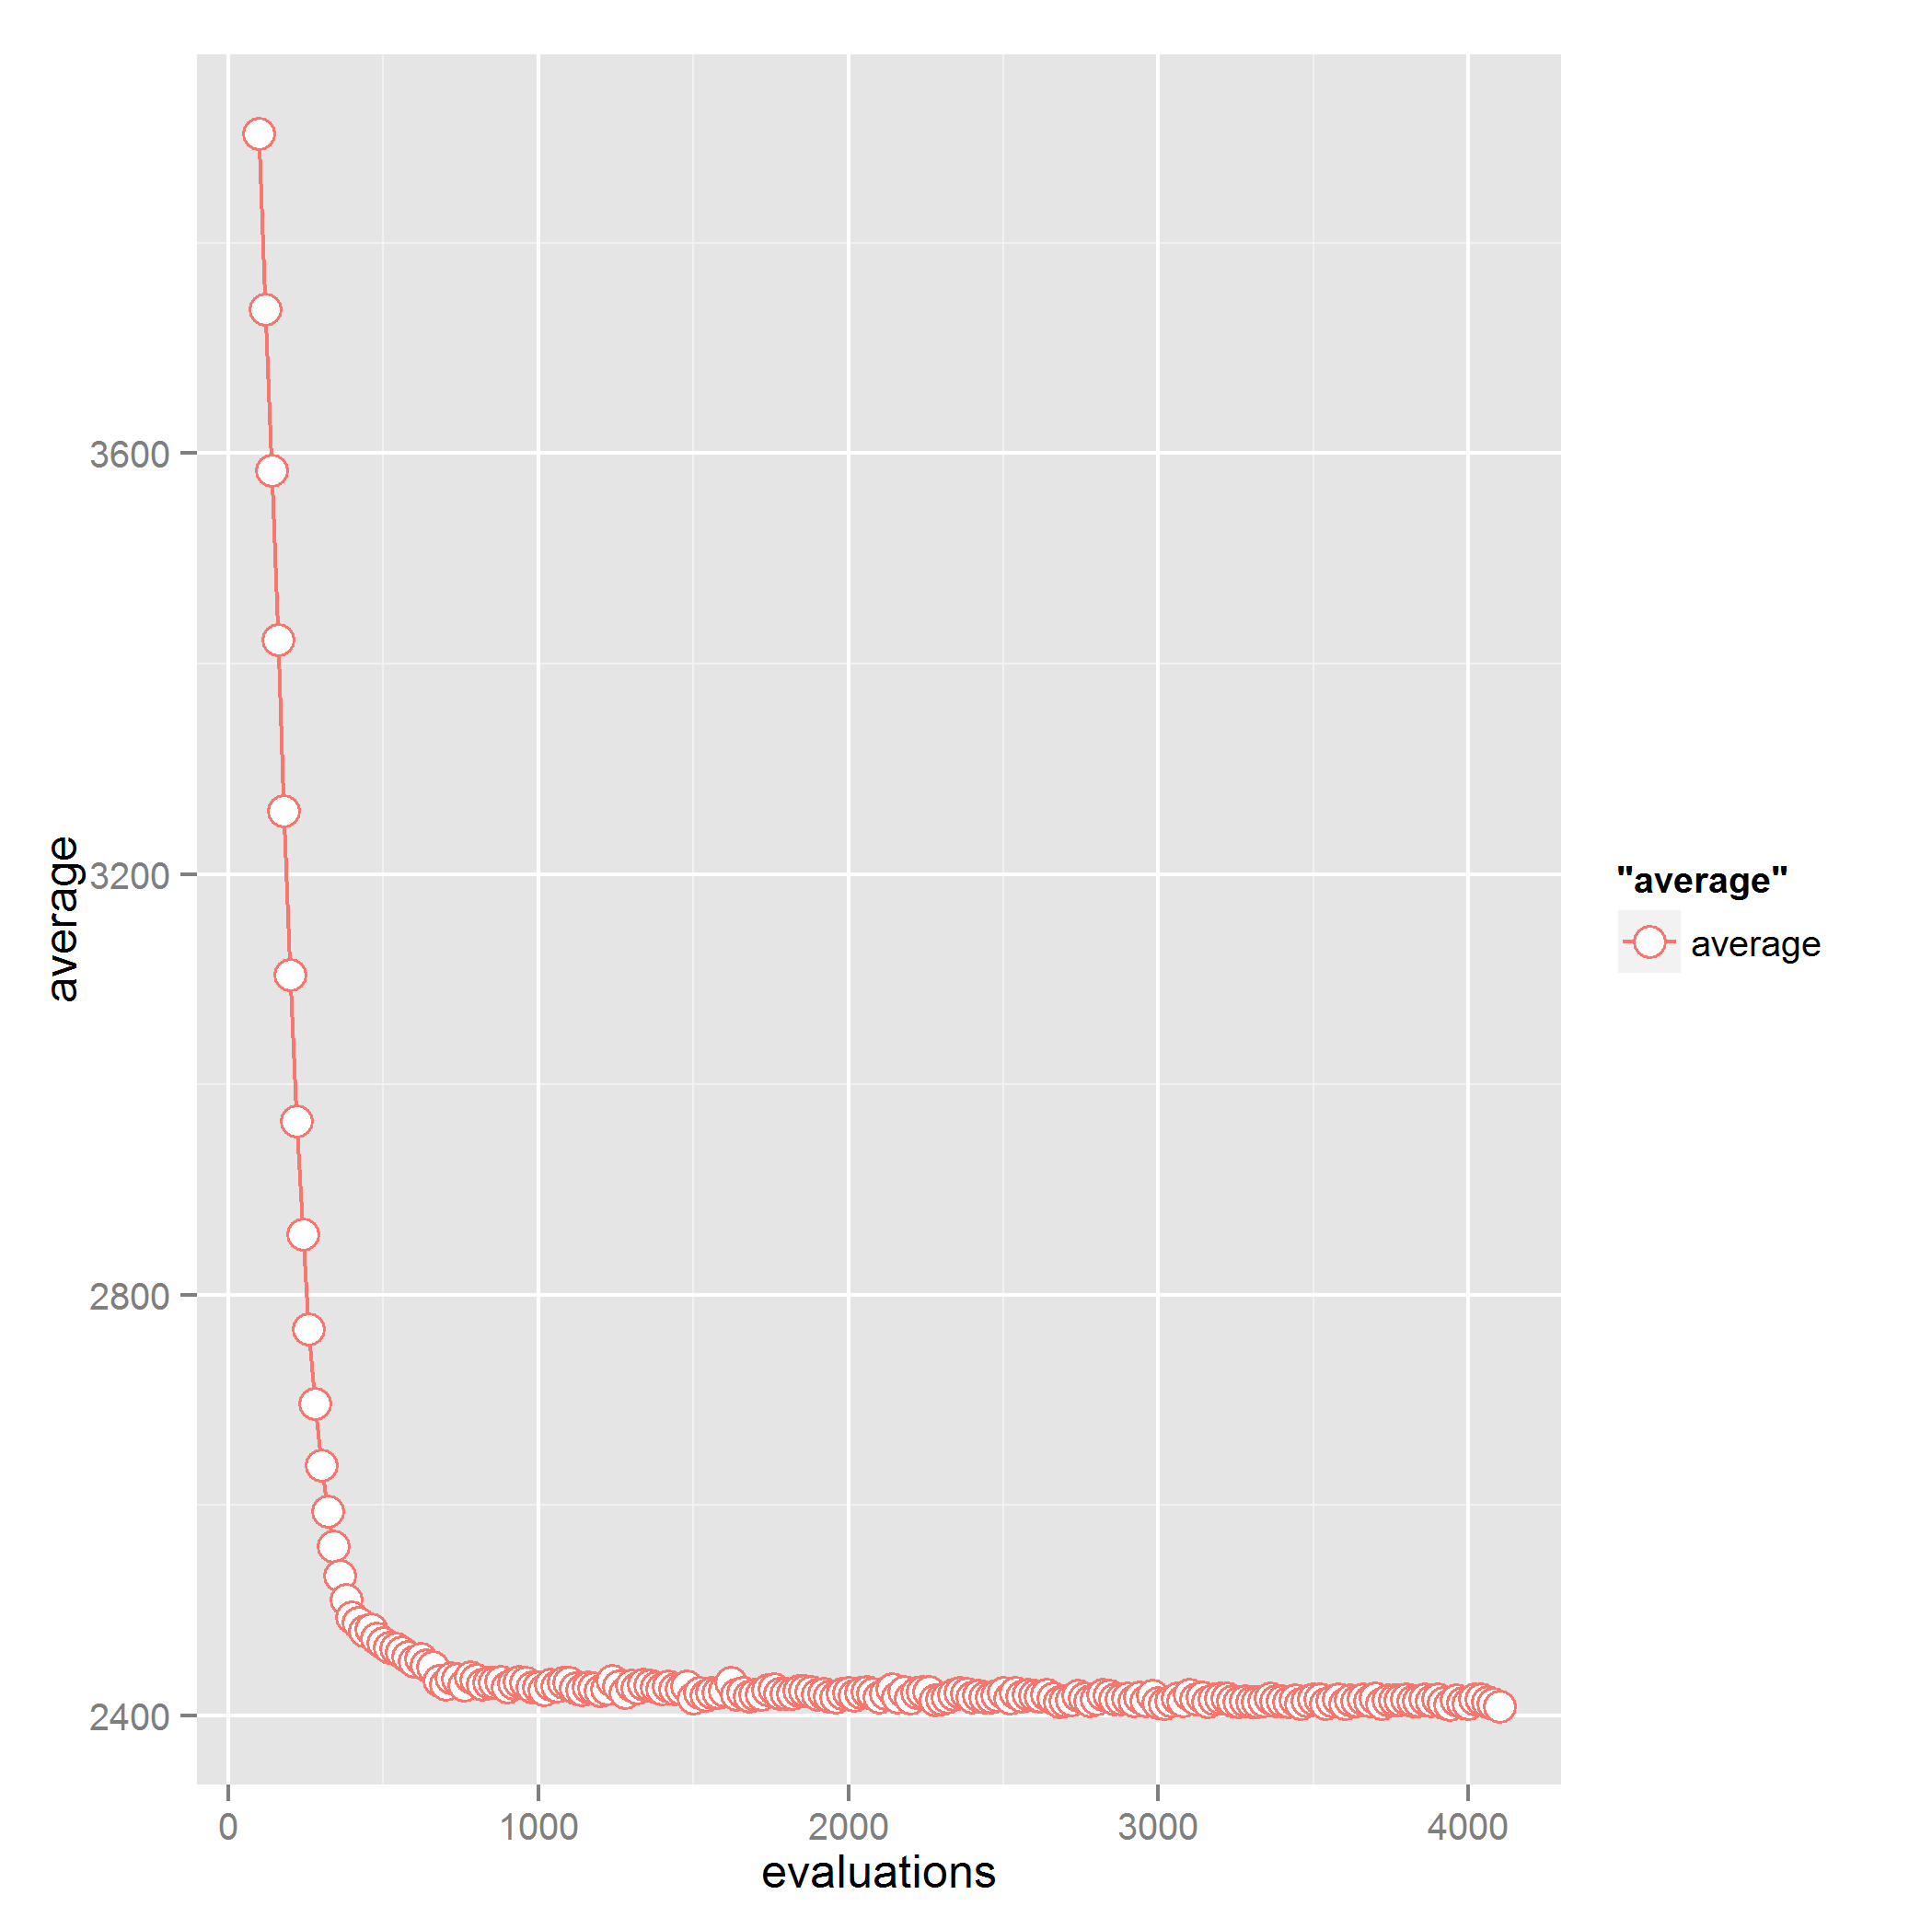
\includegraphics[]{mutation_cooling_graph0.png}

Średni rozmiar danych:

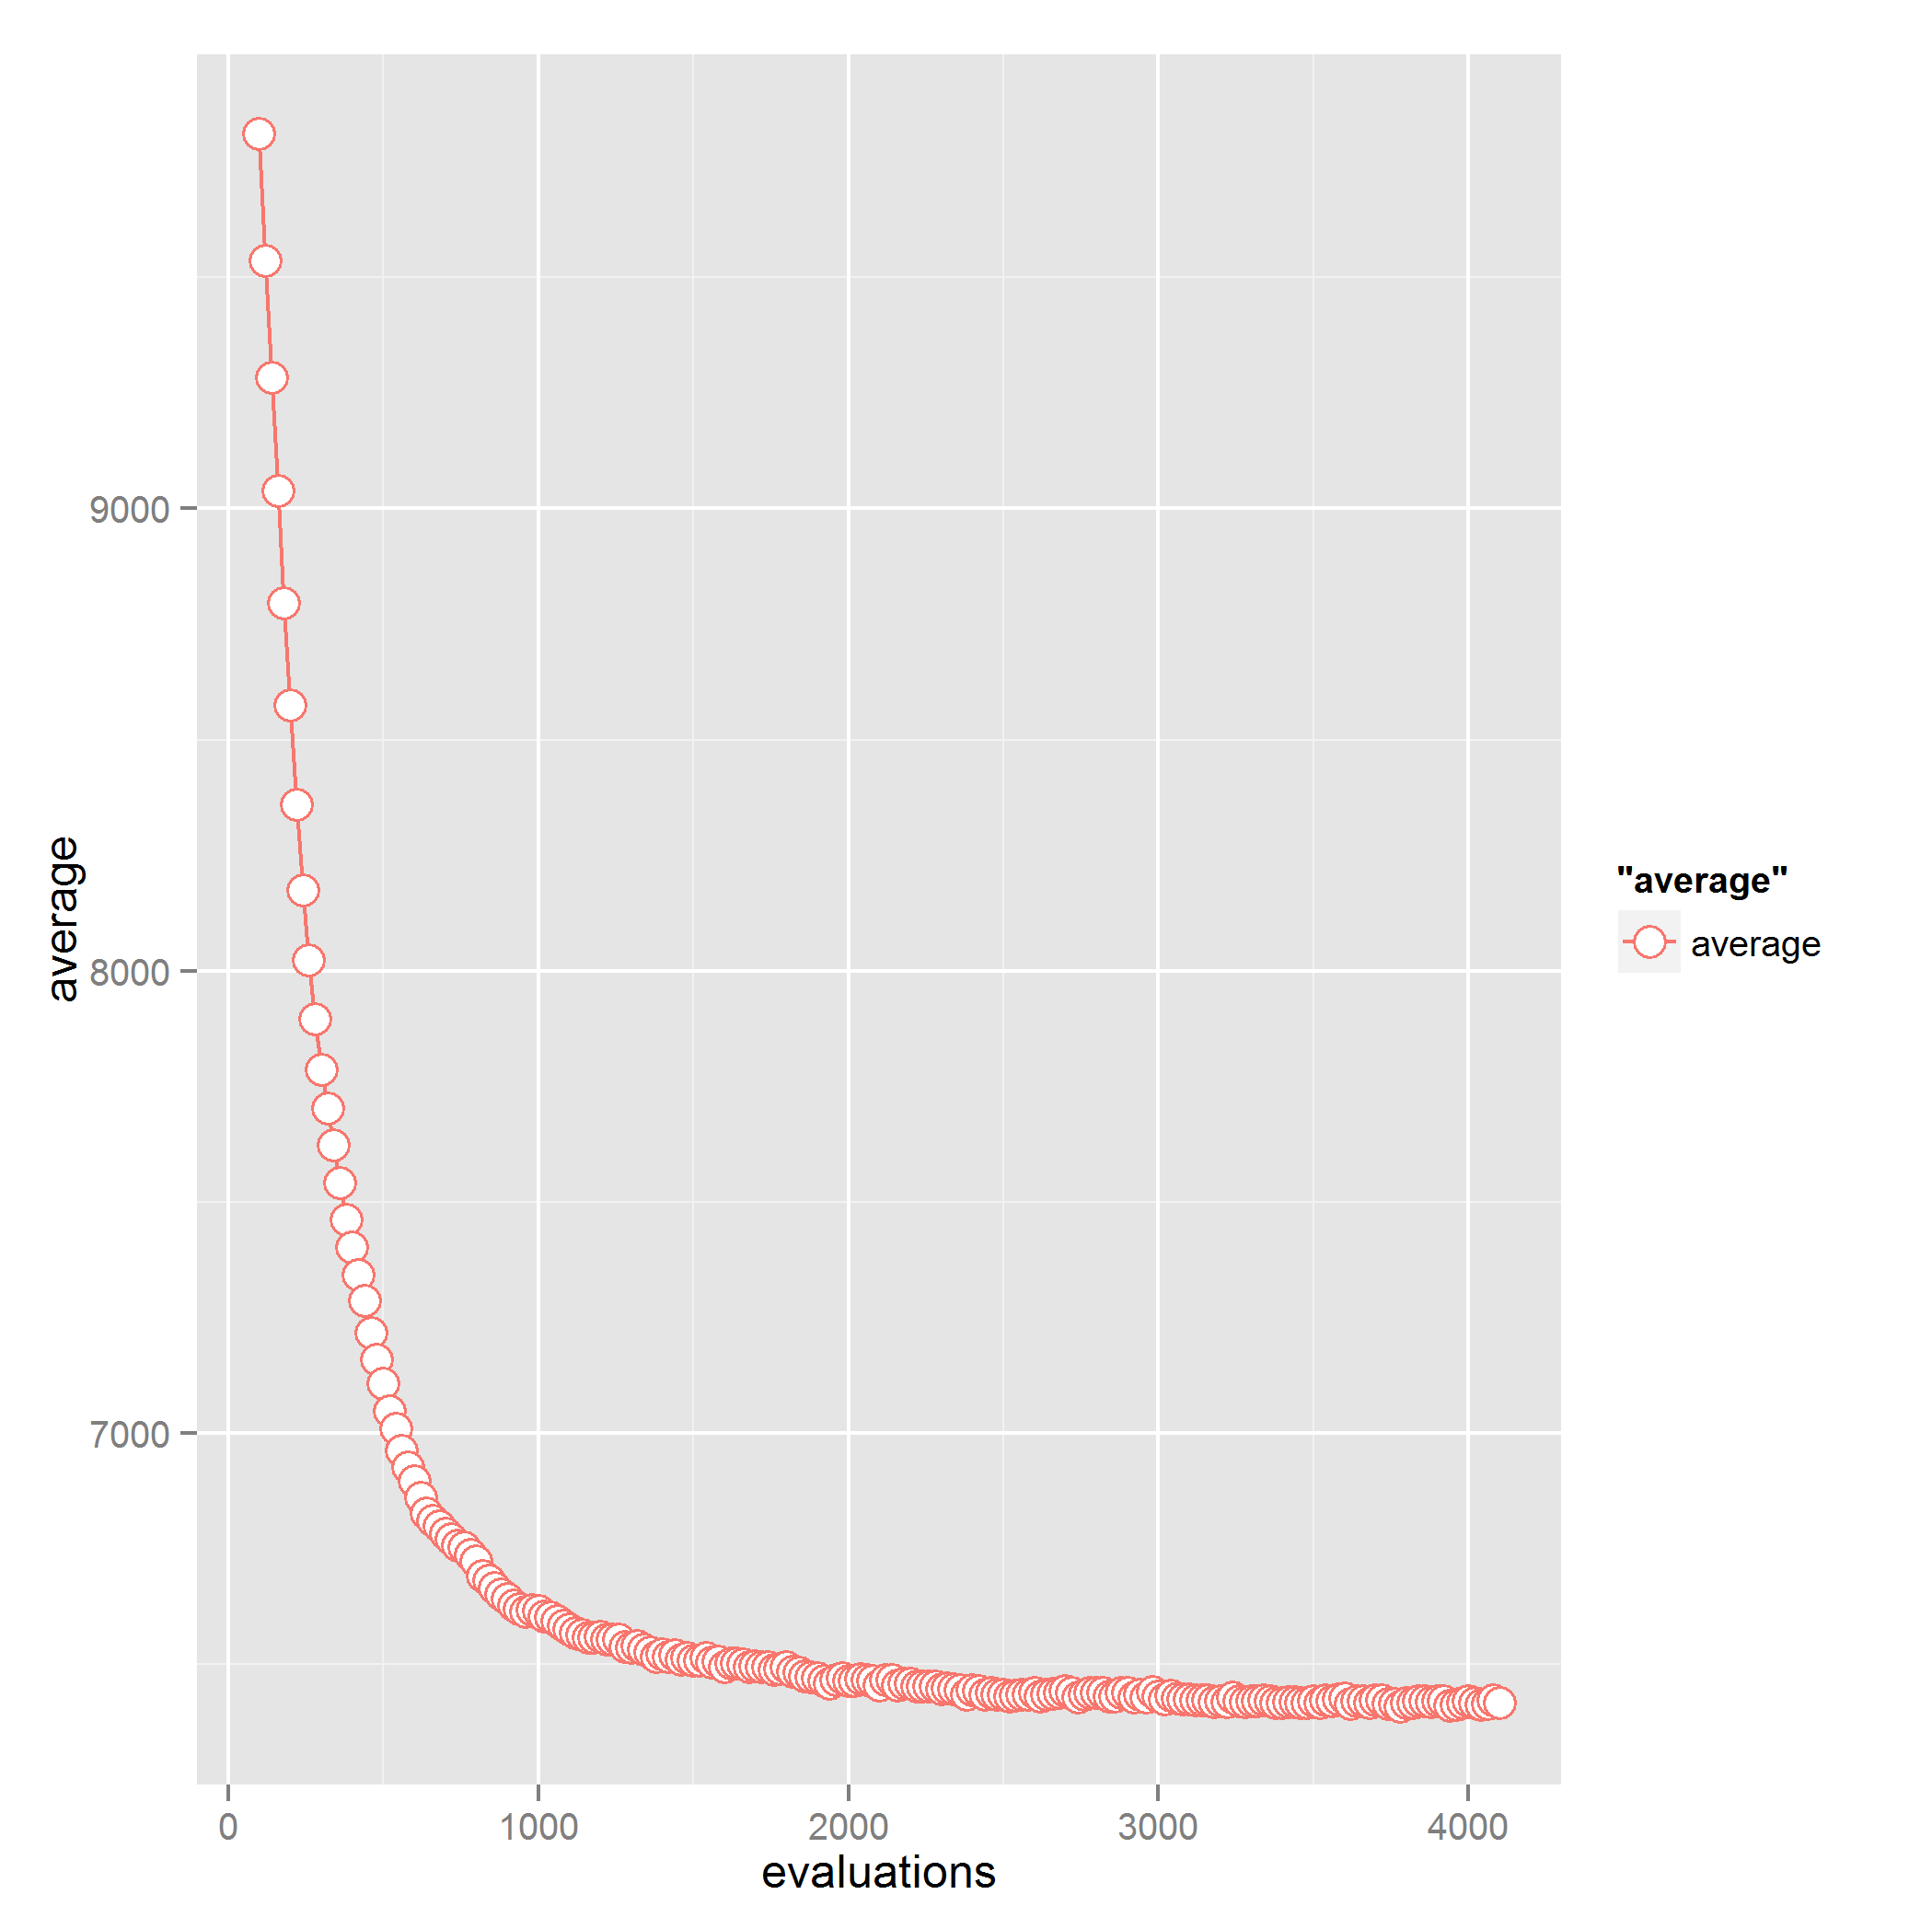
\includegraphics[]{mutation_cooling_graph1.png}

Duży rozmiar danych:

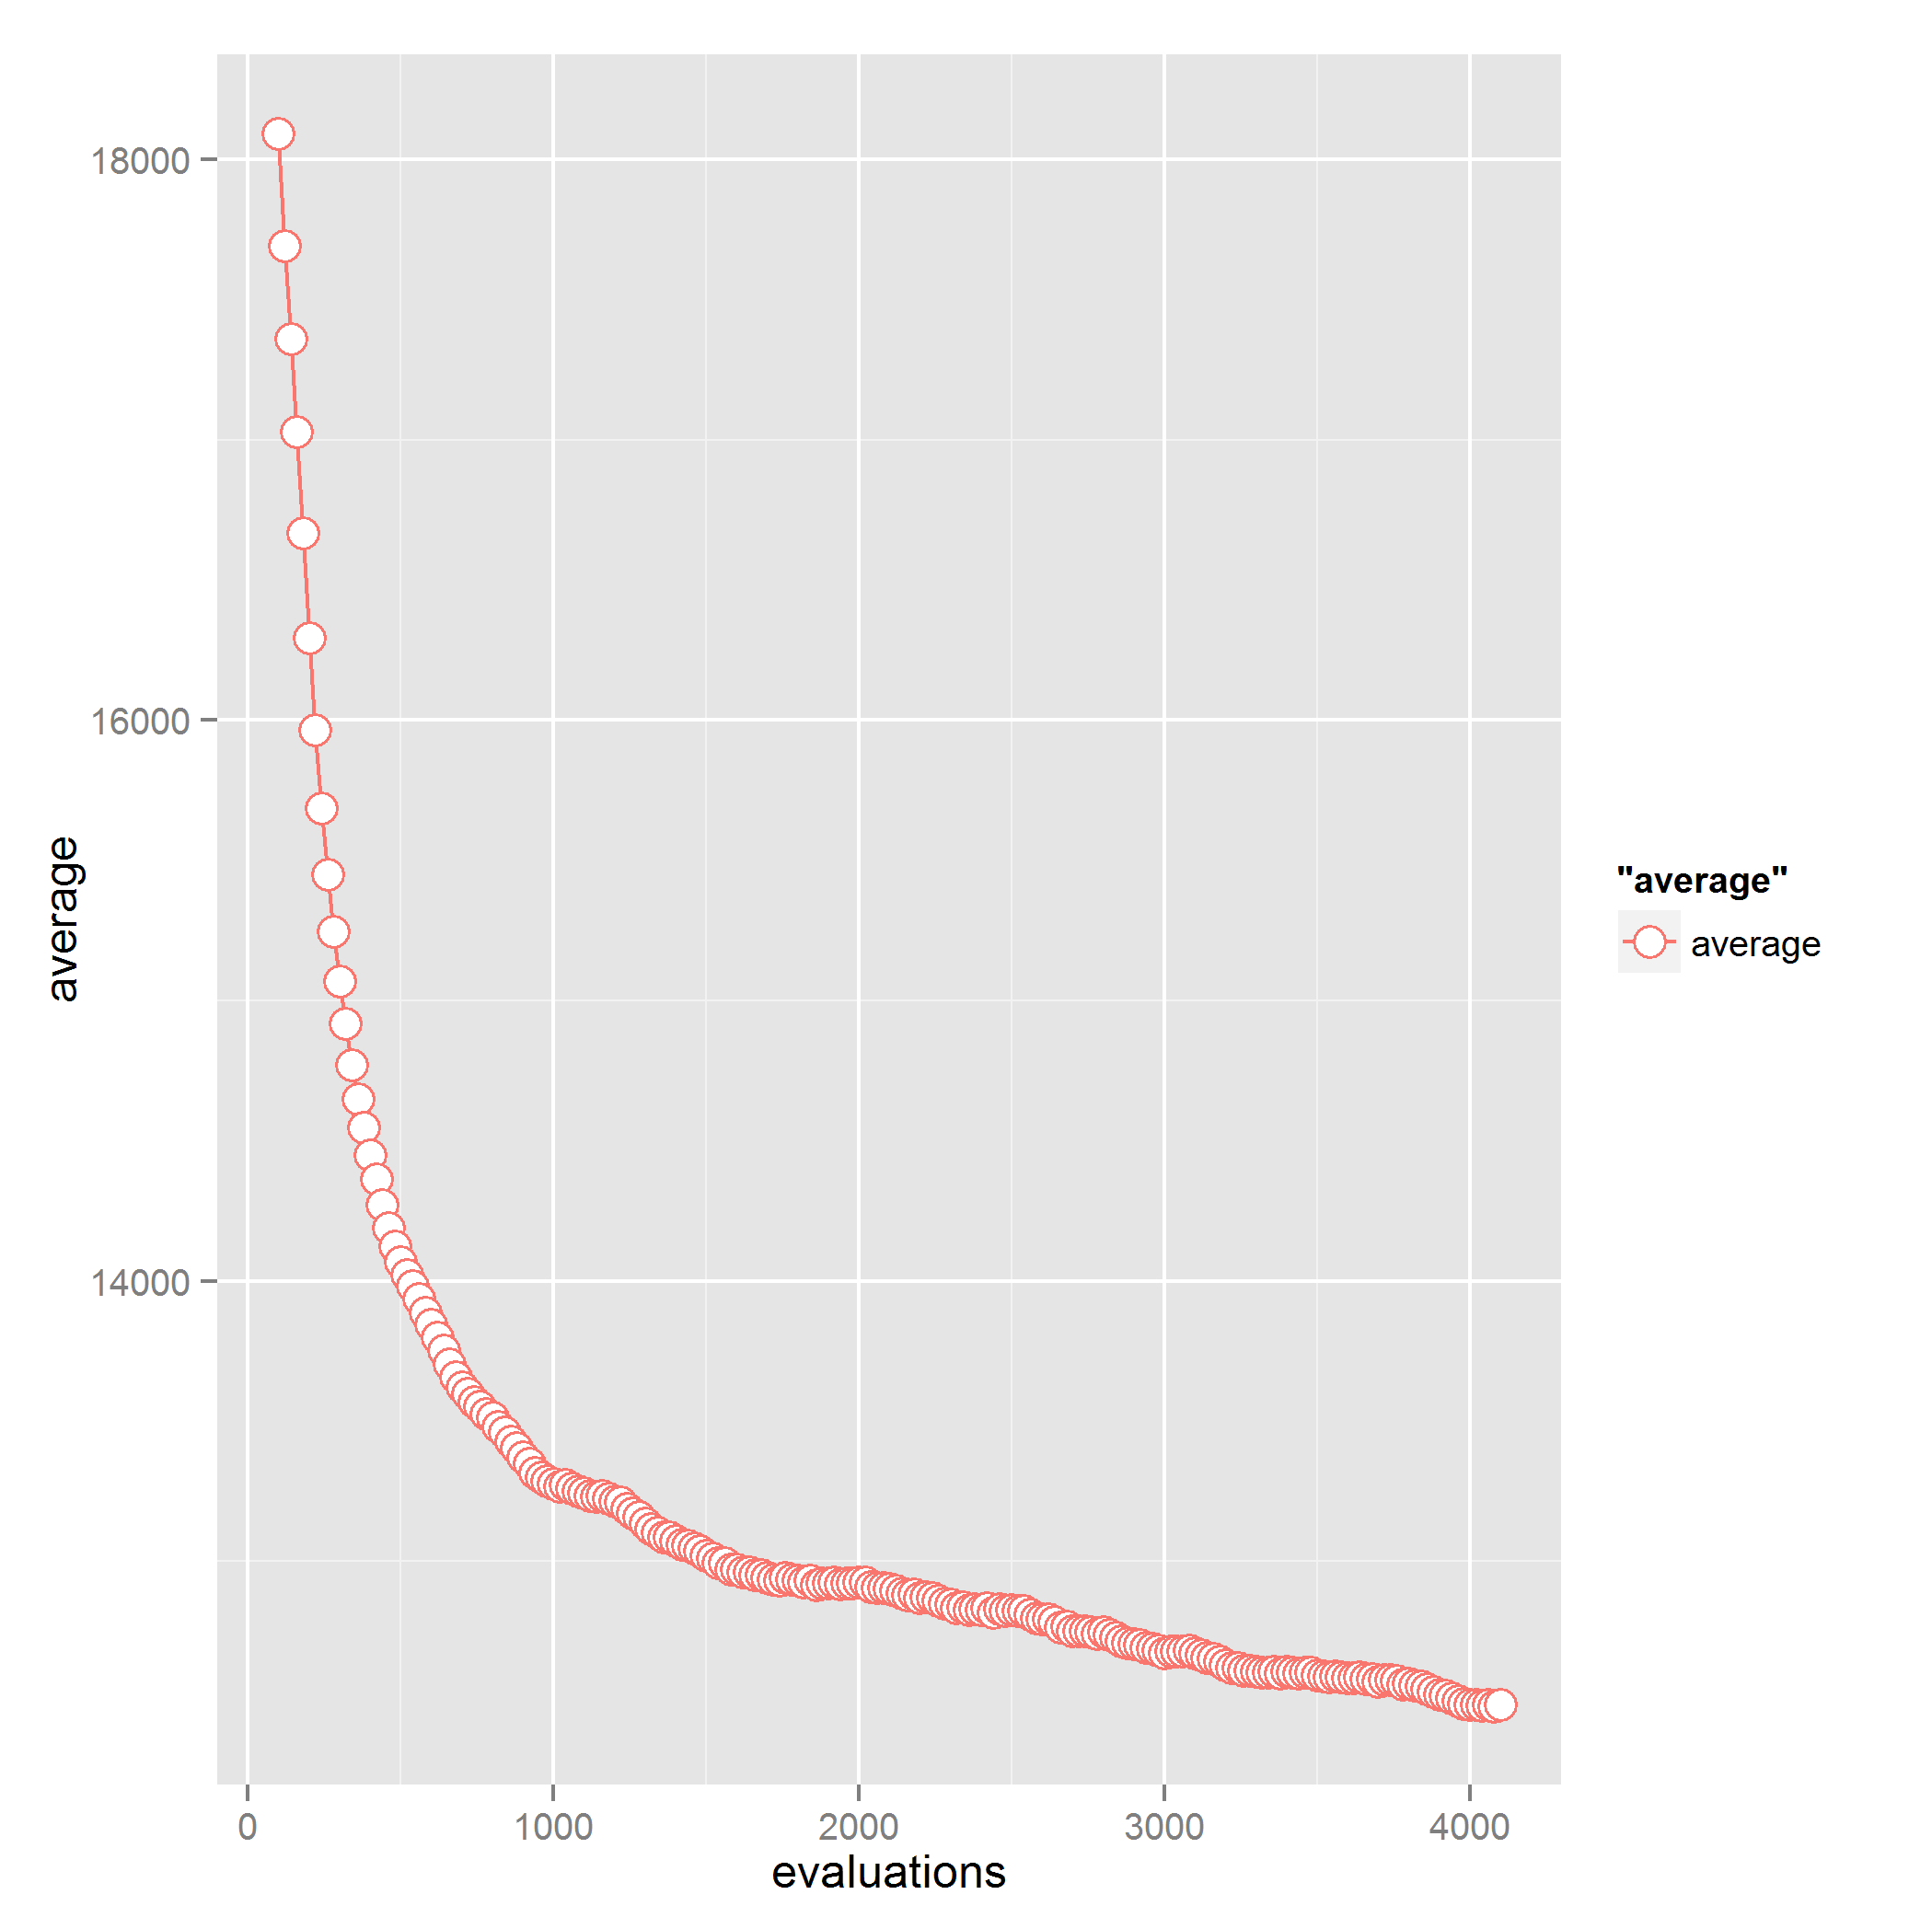
\includegraphics[]{mutation_cooling_graph2.png}

Ostatni przypadek pochodzi od hybrydy w której jako presję selekcyjną wykorzystaliśmy rozmiar turnieju. Ponieważ im większy turniej tym mniejsze prawdopodobieństwo przetrwania słabych osobników, na początku ustalilismy mały rozmiar turnieju, który stopniowo rośnie.

Mały rozmiar danych:

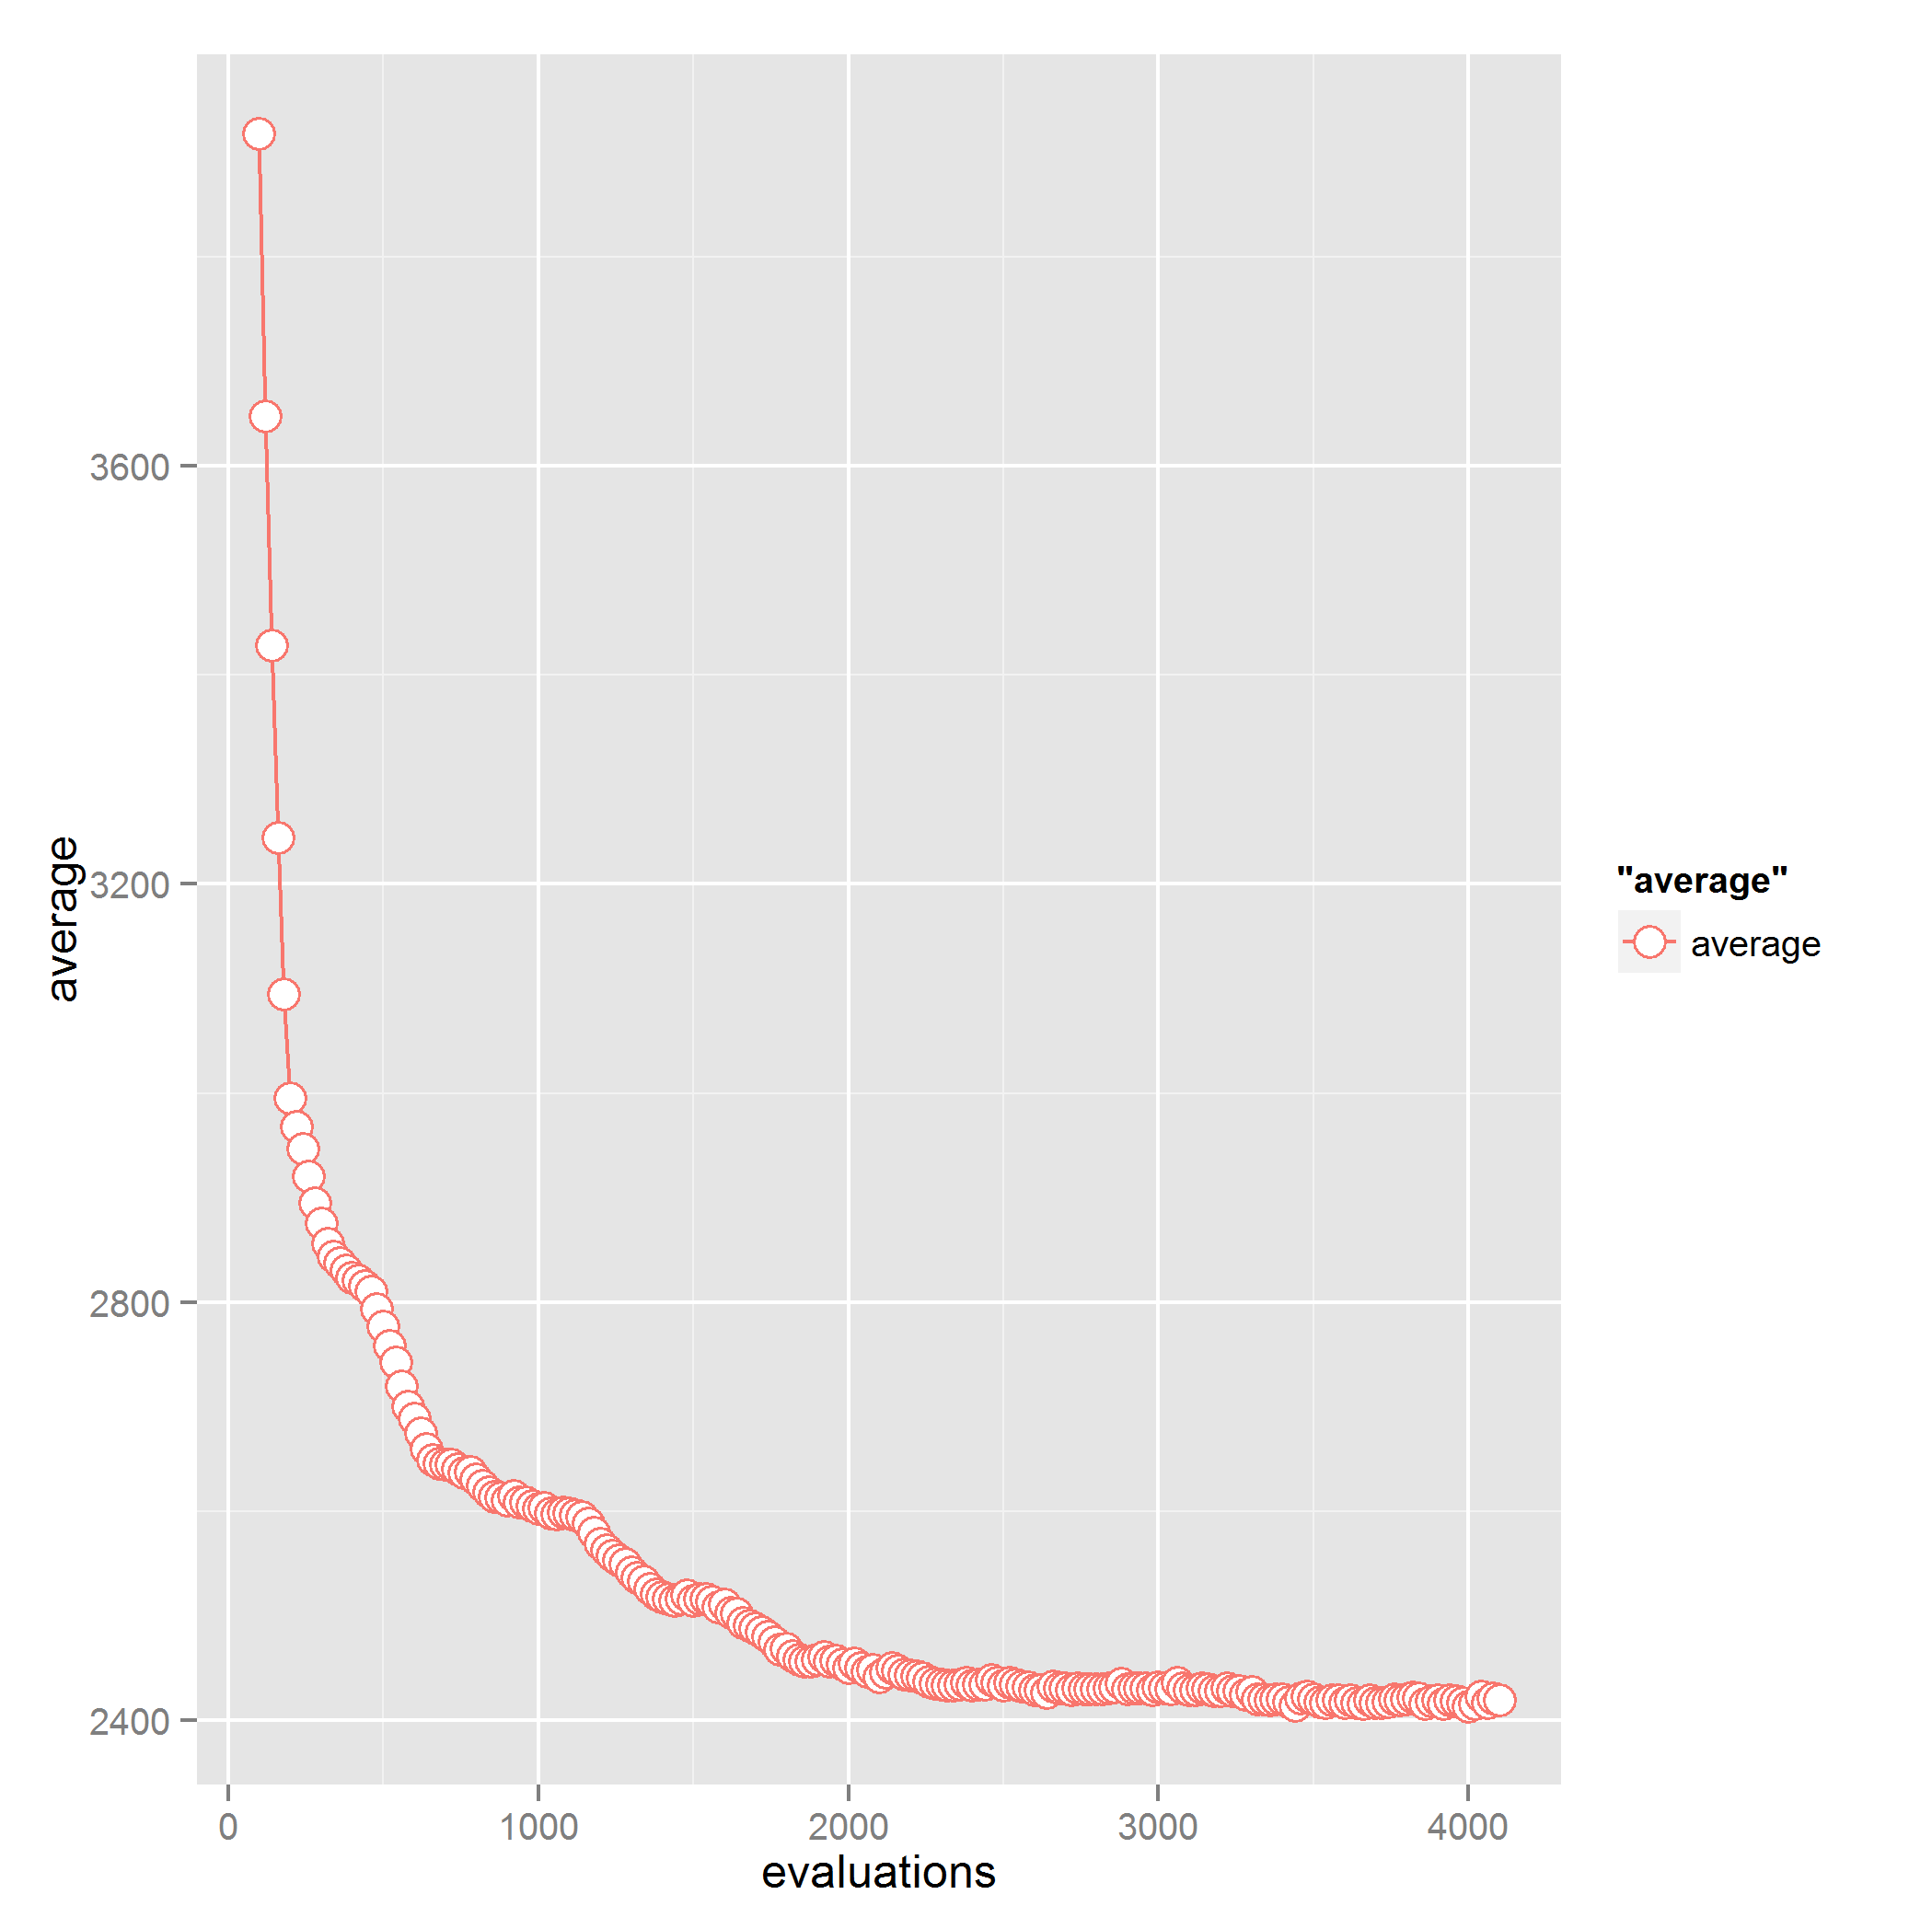
\includegraphics[]{tournament_cooling_graph0.png}

Średni rozmiar danych:

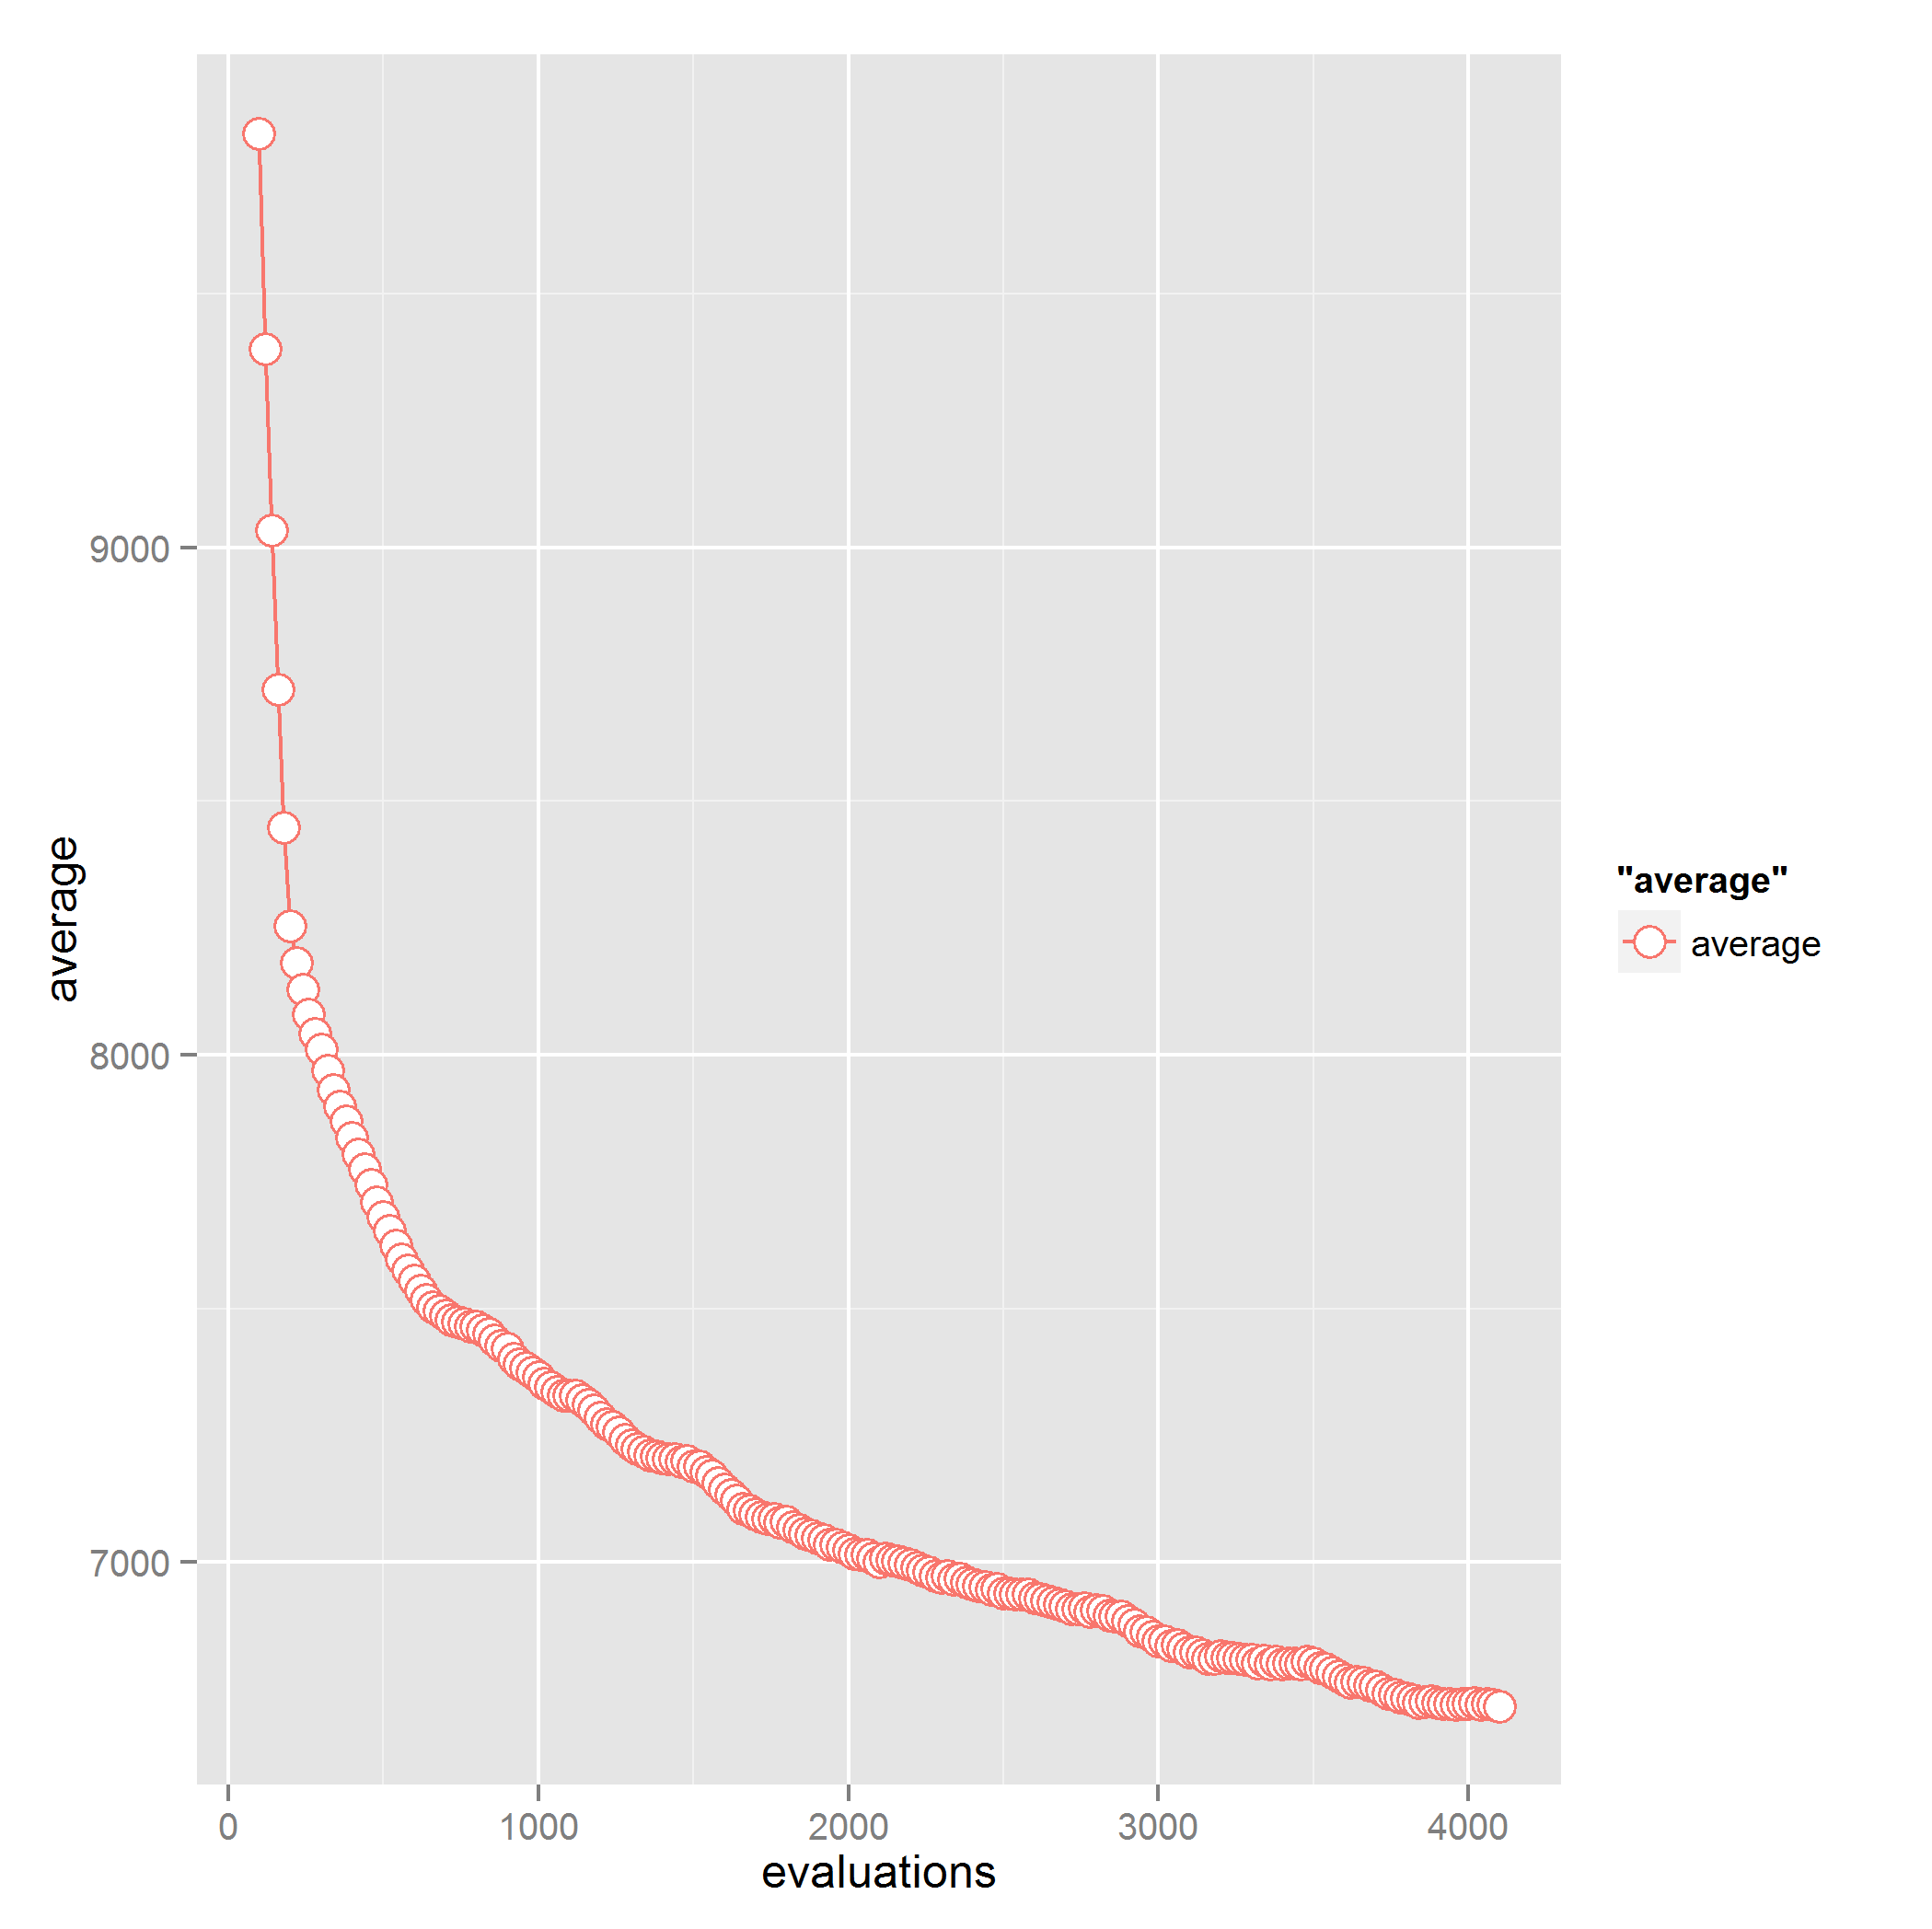
\includegraphics[]{tournament_cooling_graph1.png}

Duży rozmiar danych:

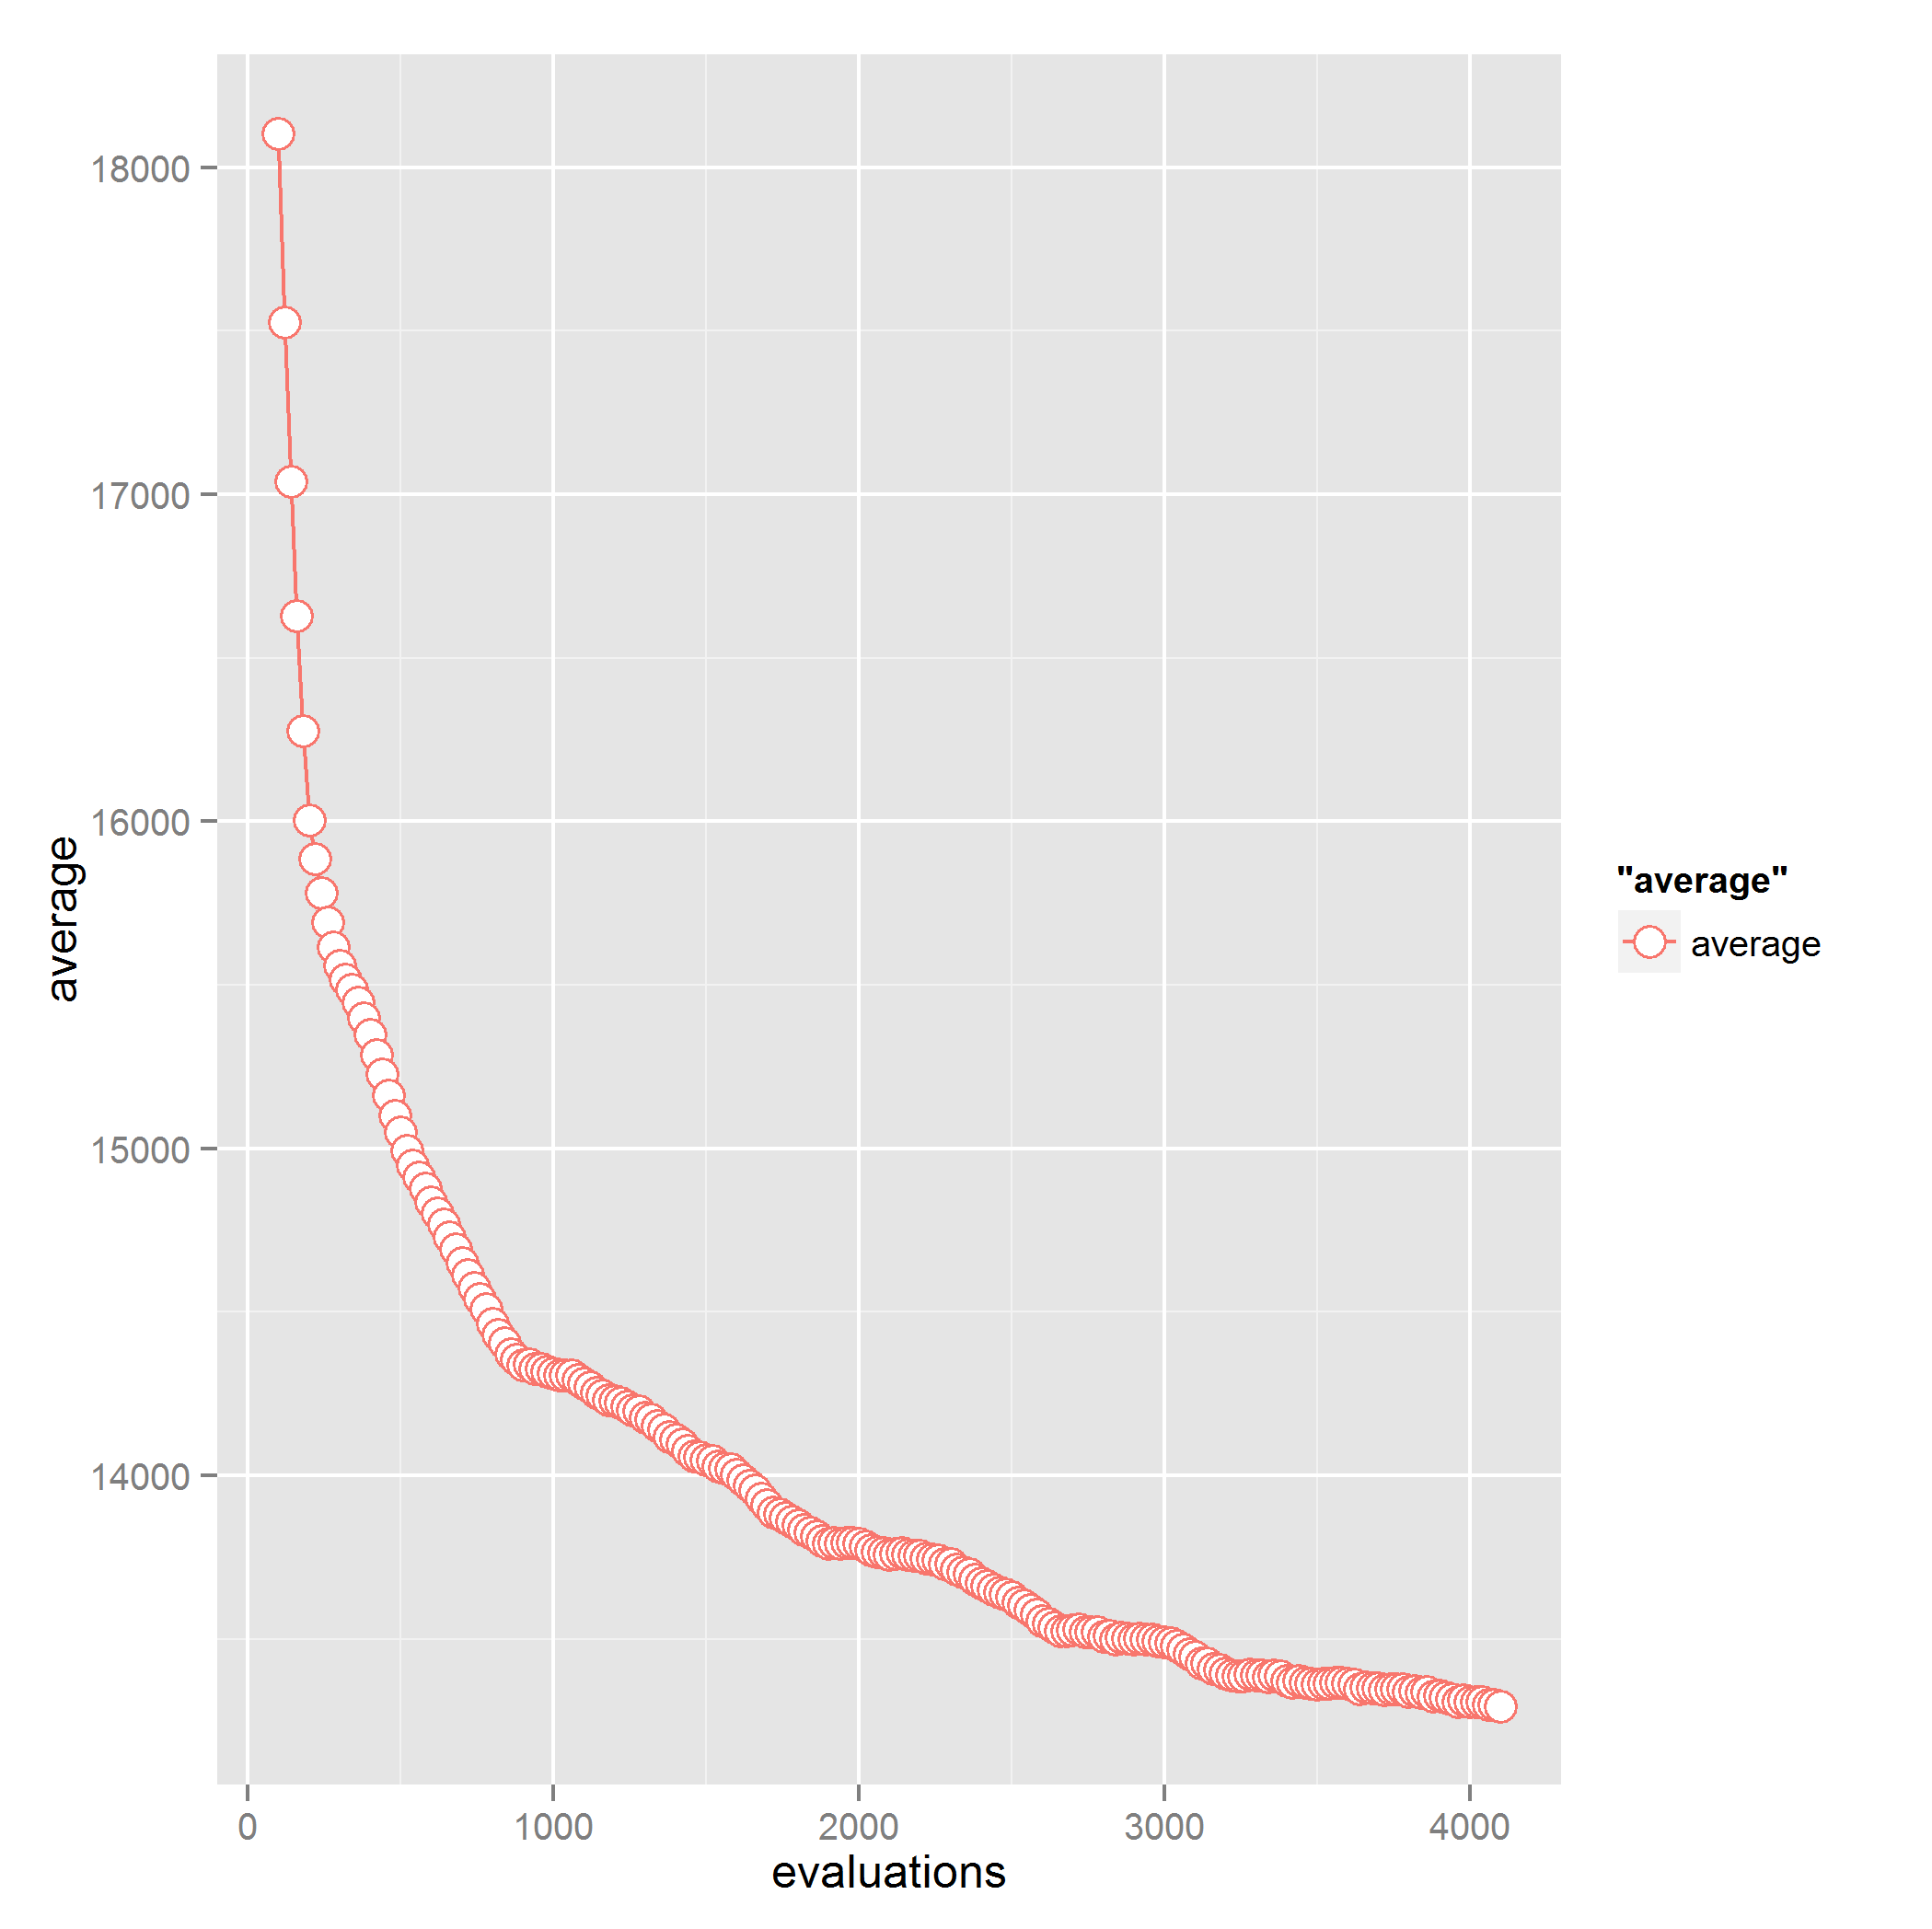
\includegraphics[]{tournament_cooling_graph2.png}

\section*{Wnioski}

Okazuje się że wbrew oczekiwaniom, najzwyklejszy algorytm genetyczny daje lepsze wyniki i jest szybciej zbieżny do optymalnego rozwiązania niż hybrydy. Obie hybrydy algorytmu genetycznego z symulowanym wyzarzaniem dają wyniki w bardzo zbliżonym czasie i są zbieżne z podobną prędkoscią. Nie jesteśmy w stanie określić jaka jest przyczyna takiego stanu rzeczy.
